\documentclass{article}
\usepackage[preprint]{caisc_2026}
\usepackage[utf8]{inputenc}
\usepackage[T1]{fontenc}
\usepackage{booktabs}
\usepackage{graphicx}
\usepackage{amsmath}
\usepackage{xcolor}
\title{When Reward-Uncertainty Coupling Cannot Be Tested: Validity Gates for DPOE}
\author{Anonymous human author\\Autoresearch artifact}
\begin{document}
\maketitle
\begin{abstract}
We stress-tested DPOE, a proposal to use one calibrated epistemic reward-uncertainty signal pessimistically for reward and policy updates and optimistically for exploration during visual-domain adaptation. On a CPU-only host, we ran two locked synthetic mechanism tests and a preregistered development solvability gate; no MLLM was run. Analytically, the frozen reward-model information-gain rationale is structurally false: visits cannot reduce uncertainty in a frozen model. MVE 2 corroborated this diagnosis because apparent benefit followed static reward--uncertainty alignment. A coupling factorial initially produced a recorded C3 kill, but independent review exposed an exploitation floor: the policy almost never reached the true goal. We withdrew that kill and reclassified the factorial as untested. A fresh bounded v2 development grid also failed its oracle reachability/none-separation gate, with no pilot or locked-v2 seed opened. Thus C1 is untested, C2's frozen information-gain rationale is structurally killed, and C3 is untested at toy scale. The contribution is a validity procedure, not a rescue claim.
\end{abstract}

\section{Introduction}
DPOE (Doubly Pessimistic and Optimistic Exploration) proposed using one calibrated epistemic reward-uncertainty signal to downweight reward, tighten a trust region, and guide optimistic state collection. This artifact does not validate that proposal. It reports a bounded, auditable stress test designed to reveal where its claims fail to be testable.

The available machine had four CPU cores, 5.8 GiB RAM, and no accessible GPU. The experiments are therefore synthetic visual mechanism tests, not evidence about MLLMs, robot control, or real visual domain shift. Recent work also narrows the original novelty: specialized small reward models can outperform larger models, so a generic small-beats-large result would not isolate calibration from specialization, data, regularization, or reward scale \citep{drivereward}. Uncertainty-weighted pessimism and visual reward-guided RL are also crowded areas \citep{hahami,vlmar3l,largereward}.

\section{Related work}

VPO chooses optimism for online RLHF and pessimism for offline RLHF through sign-modulated value regularization; DPOE's proposed delta was simultaneous pessimistic exploitation and optimistic collection from one signal inside one visual-adaptation loop \citep{cen}. Park et al. calibrate process-reward success probabilities and confidence bounds for inference-compute allocation, not RL-time adaptation \citep{park}. Pessimistic reward-model use is already represented by ensemble conservative objectives, uncertainty-penalized LoRA ensembles, and adversarial preference optimization \citep{coste,zhai,kang}. These works mean neither pessimism nor calibration alone is a DPOE novelty.

For optimism, Liang et al. use reward-ensemble disagreement as an exploration bonus in preference-based robot learning \citep{liang}. Li et al. show that naive additive bonuses under KL or alpha-divergence regularization can bias sampling toward high-reference-probability regions and propose a reference-dependent correction \citep{li}; this makes naive UCB an inadequate future baseline. Kendall and Gal motivate the epistemic/aleatoric vocabulary \citep{kendall}, but heterogeneous-feedback modeling cautions against treating ensemble disagreement as a clean decomposition \citep{liu}. DriveReward further weakens the broad surprise that a small reward model can beat larger VLMs because specialization and data are competing explanations \citep{drivereward}. The sprint therefore tests a narrow mechanism claim rather than claiming these ingredients as new.

\section{Claims and scope}
\begin{table}[t]
\caption{Closed-sprint claim table. Killed is used only for the frozen information-gain rationale, not for the broader empirical hypothesis.}
\label{tab:claims}
\centering
\small
\begin{tabular}{p{0.17\linewidth}p{0.74\linewidth}}
\toprule
Claim & Closed-sprint status \\
\midrule
C1: calibration $>$ capacity & \textbf{Untested.} MVE 1 did not run. DriveReward means any future C1 test must control specialization, data, reward scale, calibrated-large, and matched compute. \\
C2: epistemic is the signal & \textbf{Frozen information-gain rationale structurally killed analytically and corroborated by MVE 2.} A frozen reward model cannot learn from policy visits. The broader online-estimator claim is unresolved because the tested bootstrap disagreement barely predicted target error. \\
C3: coupled P/K/O & \textbf{Untested at toy scale.} v1 had an exploitation design floor. v2 was \emph{not solvable within the preregistered grid}; it did not open pilot/locked-v2 seeds. \\
\bottomrule
\end{tabular}
\end{table}

This paper therefore makes a methods claim, not a rescue claim: a factorial comparison does not answer a mechanism question unless the policy can act on a known goal and the putative uncertainty signal is valid for the intended use.

\section{Methods}
\subsection{MVE 2: frozen versus online reward uncertainty}
MVE 2 used a NumPy procedural visual contextual bandit with three shifts, 50 untouched locked seeds, aligned/decorrelated/anti-correlated reward--uncertainty layouts, and seven signals: epistemic, aleatoric, total, point, shuffled, matched-uniform, and count. Frozen and online reward-model regimes were separated. The bootstrap-linear epistemic estimator was checked on held-out shifted points before downstream outcomes were interpreted. Paired bootstrap intervals are reported; this was a toy mechanism test rather than an MLLM experiment.

\subsection{MVE 3: coupling factorial and validity gates}
MVE 3 v1 used a binary-tree visual gridworld with an online conjugate reward posterior, separate collection and evaluation, 50 locked paired replicates, three severities, four signal-quality tiers, and the complete $P\times K\times O$ factorial. Controlled uncertainty passed quality and leakage checks; learned bootstrap did not. The locked analysis used simultaneous bootstrap intervals and Holm-adjusted tests.

After independent review found that exploitation was essentially unable to reach the goal, v2 preregistered a fresh development-only 27-tuple grid over reference temperature, trust-region coefficient, and reward clip. Its oracle-versus-none gate required aggregate oracle success $\geq25\%$, each severity $\geq15\%$, an oracle-minus-none success gap $\geq15$ percentage points, and return-AUC separation $\geq0.10$. Passing would have been required before an adaptation-engagement gate, pilot, or fresh locked seeds.

\section{Results}
\subsection{C2: the frozen mechanism is structurally wrong}
The frozen arm cannot implement information gain: reward-model parameters do not change, so visits cannot reduce epistemic uncertainty. On the correlation-neutral layout, epistemic minus point was $-0.0036$ (95\% CI $[-0.0073,0.0003]$). It was $+0.0719$ under aligned layouts and $-0.0719$ under rank-reversed anti layouts. Apparent benefit tracked a static prior that pointed toward reward, not acquired information. Online, epistemic beat aleatoric by $+0.0081$ (95\% CI $[0.0030,0.0131]$, $d_z=0.60$), the one contrast pointing toward C2, but it tied total and lost to several generic controls. Because the estimator was weak (error AUROC 0.532; Spearman 0.162), neither the favorable contrast nor the broader online outcome cleanly adjudicates the stronger hypothesis.

\subsection{C3 v1: a recorded kill was withdrawn}
The controlled v1 signal passed locked quality checks (AUROC 0.850--0.924; Spearman 0.647--0.710) and the leakage guard (partial Spearman 0.0124). Full P+K+O lost to O by $-0.0021$ return AUC (simultaneous CI $[-0.0058,-0.0002]$) and to P+O by $-0.0050$ ($[-0.0130,-0.0005]$); the three-way interaction was approximately zero. The preregistered rule therefore produced and recorded \emph{killed-at-toy-scale}. A post-review diagnostic then found controlled true-goal-success AUC of only 0.0004 (P+K+O: 0.0002), with 98.7\% of cells at or below 0.005. Because the rule's reachable-goal premise failed, the kill was withdrawn and replaced by \emph{untested-design-floor-policy-collapse}. This is a post-review validity amendment, not a favorable reinterpretation.

\begin{figure}[t]
\centering
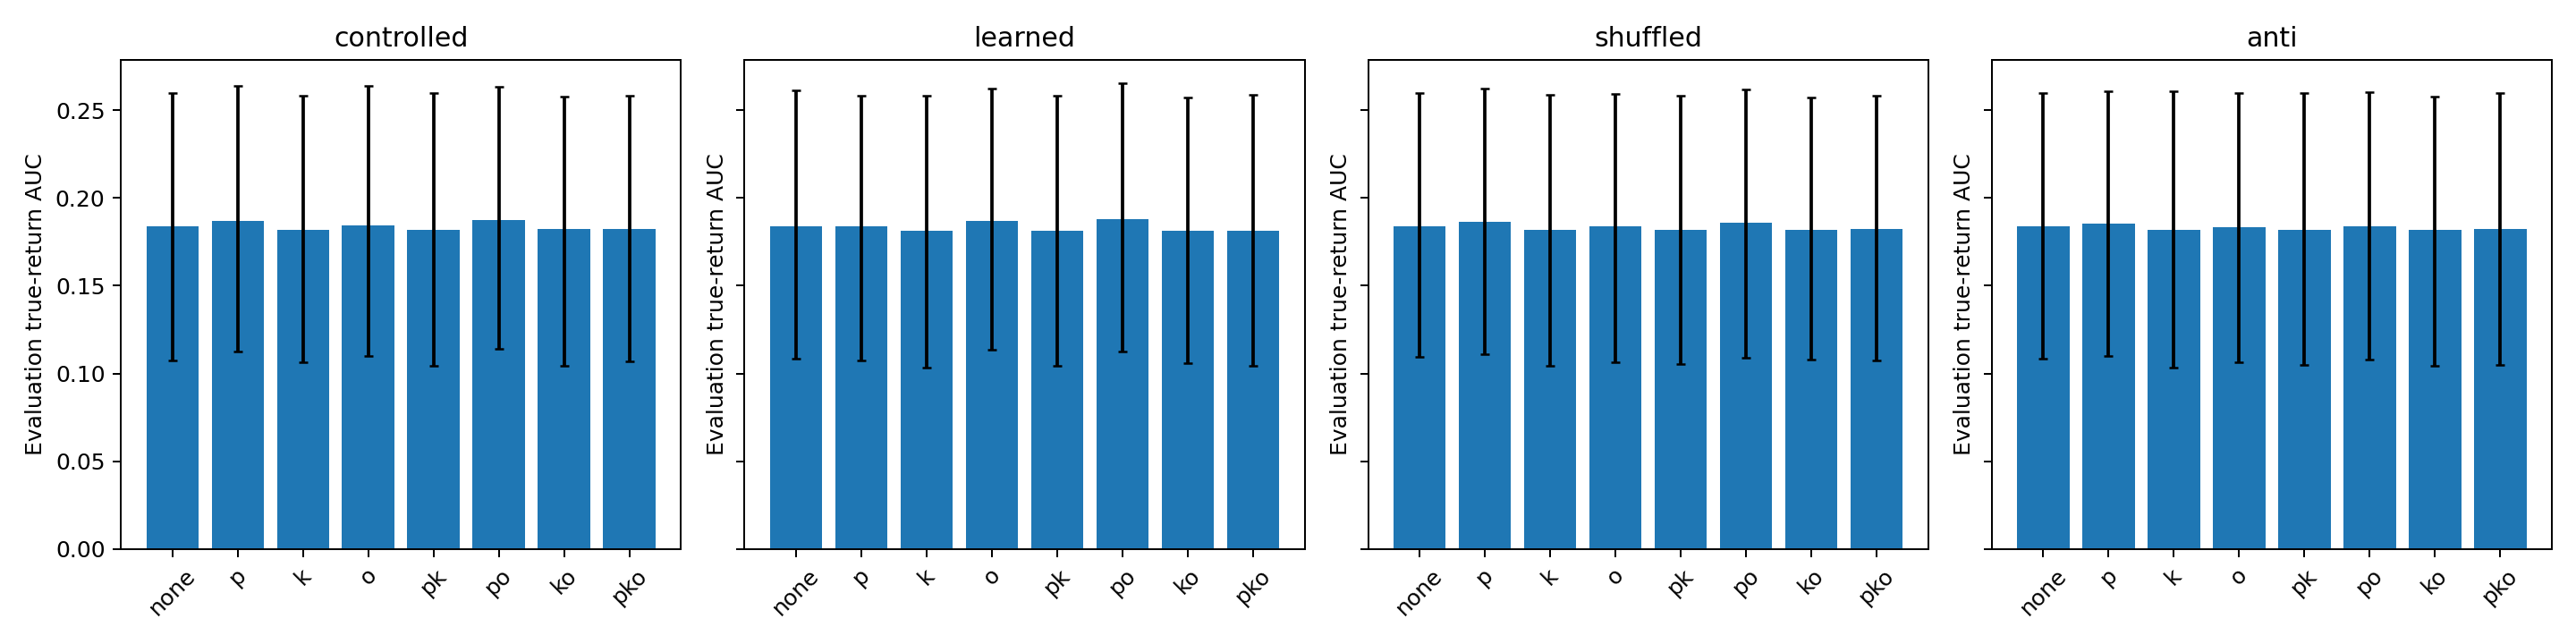
\includegraphics[width=0.95\linewidth]{mve3_return_auc_factorial.png}
\caption{Locked v1 return-AUC factorial contrasts. Retained for audit, but not a coupling null: the exploitation manipulation check failed.}
\label{fig:v1}
\end{figure}

\subsection{C3 v2: no valid factorial was opened}
The complete development grid failed before any v2 factorial. The best oracle-reachability tuple ($\tau_{\rm ref}=0.18$, $\beta_0=0.10$, clip $\pm1.75$) achieved 16.44\% aggregate oracle goal success (14.53/15.60/19.19\% by severity) and an 11.36-pp oracle-minus-none gap. It passed return-AUC separation (0.3485; 0.3142/0.2891/0.4422 by severity) but missed the two success gates. The best tuple lay on the relaxation boundary. The conclusion is \textbf{not solvable within the preregistered grid}, not globally unsolvable. The protocol barred grid extension, retuning, pilot, and locked-v2 work without a new protocol, independent review, and human sign-off.

\section{Deviations, limitations, and implications}
Seven experimental and reporting deviations are material. (1) v1's preregistered kill was withdrawn by a disclosed post-review validity amendment after its reachability premise failed. (2) The v1 locked quality gate was implemented per severity where the preregistration specified an aggregate gate; this was stricter and all controlled severities passed. (3) Learned-tier uncertainty was RMS-rescaled to controlled prior uncertainty using generator $u_0$, exposing oracle-scale information; that tier failed its quality gate and supports no claim. (4) The v2 implementation initially included a non-binding fifth source-competence guard although the written development gate listed four conditions; its minimum was 0.988 and the code was aligned to the written gate. (5) The costliest-tuple timing pre-check was skipped before the completed v2 grid. (6) The v2 artifact was regenerated report-only to add per-severity return-AUC fields; all pre-existing metric fields had identical SHA-256 fingerprints before and after. (7) The driver reported four Review-13 safeguards as applied without checking the actual failure path and persisted artifact; the audit log was corrected and Review 14 required the missing changes. None of these events authorizes a new experiment.

Reviewer provenance also matters. Reviews 01--08 and 10--13 produced usable automated CLI verdicts; Reviews 09 and 14--16 were supplied through human-mediated manual runs after repeated empty or API-error captures. The first two automated Review-16 requests for this plan and paper failed. The manual Review 16 then returned REVISE and identified the related-work, disclosure, framing, and compilation defects corrected in this version. Review 15 itself was REVISE, not the previously reported APPROVE; its remaining stale pilot name was corrected. This paper therefore claims reviewer assistance and a manual Review-16 pass, not an uninterrupted or independently verified final approval.

The primary limitation is external validity. These are CPU-scale synthetic environments, not MLLM reward models or physical domains. C1 was never tested. C2's broader online estimator claim remains unresolved. C3 has no valid toy-scale factorial conclusion. The positive contribution is a decision procedure: verify estimator quality, oracle reachability and return headroom, leakage, and adaptation over the reference baseline before interpreting a $P\times K\times O$ contrast. A valid future null may then be a negative result; this sprint's C3 outputs are not.

\begin{ack}
This artifact was produced by an autoresearch system: OpenAI Codex served as driver for implementation, analysis, and writing; Claude Code supplied independent review at multiple checkpoints, including human-mediated manual captures when the automated channel failed. The human supplied the submitted research plan, session-duration and execution authorizations, and manual review decisions. Claude review used the human's personal account and did not consume the sprint compute/API budget. Approximately \$20 of the \$50 ceiling was consumed by driver inference; local experiments cost \$0.
\end{ack}

\small
\begin{thebibliography}{99}
\bibitem[Cen et al.(2025)]{cen} Cen, S., et al. (2025). Value-incentivized preference optimization. arXiv:2405.19320.
\bibitem[Coste et al.(2024)]{coste} Coste, T., et al. (2024). Reward model ensembles help mitigate overoptimization. ICLR.
\bibitem[Chen et al.(2026a)]{drivereward} Chen, et al. (2026a). DriveReward. arXiv:2606.08525.
\bibitem[Chen et al.(2026b)]{vlmar3l} Chen, et al. (2026b). VLM-AR3L. arXiv:2607.00483.
\bibitem[Hahami et al.(2026)]{hahami} Hahami, et al. (2026). A unifying lens on reward uncertainty in RLHF. arXiv:2606.09073.
\bibitem[Kendall and Gal(2017)]{kendall} Kendall, A. and Gal, Y. (2017). What uncertainties do we need in Bayesian deep learning for computer vision? NeurIPS.
\bibitem[Li et al.(2026)]{li} Li, W., Oh, C., and Li, S. (2026). General exploratory bonus for optimistic exploration in RLHF. ICLR.
\bibitem[Liang et al.(2022)]{liang} Liang, X., et al. (2022). Reward uncertainty for exploration in preference-based reinforcement learning. ICLR.
\bibitem[Liu et al.(2025)]{liu} Liu, et al. (2025). Uncertainty quantification for large language model reward learning under heterogeneous human feedback. arXiv:2512.03208.
\bibitem[Park et al.(2025)]{park} Park, Y.-J., et al. (2025). Know what you don't know: uncertainty calibration of process reward models. NeurIPS.
\bibitem[Wu et al.(2026)]{largereward} Wu, et al. (2026). Large reward models. arXiv:2603.16065.
\bibitem[Zhai et al.(2024)]{zhai} Zhai, Y., et al. (2024). Uncertainty-penalized RLHF with diverse reward LoRA ensembles. arXiv:2401.00243.
\bibitem[Kang and Oh(2025)]{kang} Kang, H. and Oh, M. (2025). Adversarial policy optimization for offline preference-based reinforcement learning. ICLR. arXiv:2503.05306.
\end{thebibliography}

\appendix
\section{Closed experiment record}
MVE 2 used 6,300 locked rows and completed its locked run in 257.7 seconds. MVE 3 v1 completed 4,800/4,800 locked cells and its integrity audit found no missing, invalid, temporary, pairing, or scenario-violation files. Its local locked execution took 8,462.3 seconds. MVE 3 v2 opened only the development-v2 namespace. Its report-only regeneration neither selected nor retuned a tuple and opened no pilot/locked-v2 seed. The repository retains manifests, raw cells, reports, tests, and review artifacts.

\section{Preregistration audit}
The v1 factor parser bug was caught in a debugging pilot before lock; the paired corrected v1 pilot was retained under a non-v2 name. Three intended MVE 2 test seeds were opened in pilot work and excluded before the confirmatory block was chosen. MVE 2 used all 160 collection episodes for its hacking denominator, fitted development scales before layout permutation, and had a few target-render RNG overlaps. These are disclosed limitations, not excuses for stronger claims.

\newpage
\section*{Conference For AI Scientists 2026 - AI Involvement Checklist}
\subsection*{Research Stage Assessment}
\begin{enumerate}
\item \textbf{Hypothesis development}\\
Answer: \involvementB{} \quad Iteration Effort: \iterationLow{}\\
Explanation: The human supplied the screened DPOE plan; the driver sharpened its testable boundaries using literature and experiment evidence.
\item \textbf{Experimental design and implementation}\\
Answer: \involvementC{} \quad Iteration Effort: \iterationMedium{}\\
Explanation: The driver designed and implemented toy MVEs and audit machinery; the human authorized execution and scope changes, while AI review identified validity faults. Some later review outputs were obtained through human-mediated manual runs after the automated channel failed.
\item \textbf{Analysis of data and interpretation of results}\\
Answer: \involvementC{} \quad Iteration Effort: \iterationMedium{}\\
Explanation: The driver analyzed locked outputs; reviewer and human feedback forced the v1 floor reclassification and bounded v2 interpretation.
\item \textbf{Writing}\\
Answer: \involvementD{} \quad Iteration Effort: \iterationLow{}\\
Explanation: The autoresearch driver wrote this unedited first-draft paper.
\end{enumerate}
\subsection*{AI System Documentation}
\begin{enumerate}
\setcounter{enumi}{4}
\item \textbf{AI systems used}\\
Description: A frontier language-model coding agent drove local implementation, analysis, and writing; a separate frontier coding agent reviewed critical checkpoints. Some review calls returned empty or API-error captures, after which the human supplied manual runs. Specific product names are disclosed in the acknowledgments for this preprint artifact.
\item \textbf{Observed AI Limitations}\\
Description: The driver initially marked safeguards applied without checking the failure-path artifact, and it required reviewer feedback to recognize an uninformative factorial floor. Automated reviewer availability failed repeatedly; Reviews 09 and 14--16 were human-mediated manual outputs, and Review 15 had first been misreported as APPROVE although its saved verdict was REVISE. These limitations are retained in the audit trail.
\end{enumerate}

\newpage
\section*{Conference For AI Scientists 2026 - Reproducibility and Responsibility Checklist}
\begin{enumerate}
\item \textbf{Claims}\\ Answer: \answerYes{}\\ Justification: The abstract and Table~\ref{tab:claims} separate killed, untested, and bounded conclusions.
\item \textbf{Limitations}\\ Answer: \answerYes{}\\ Justification: The limitations section states the synthetic, CPU-only, non-MLLM scope and material validity/protocol limitations.
\item \textbf{Theory assumptions and proofs}\\ Answer: \answerNA{}\\ Justification: This paper makes no theoretical result.
\item \textbf{Experimental result reproducibility}\\ Answer: \answerYes{}\\ Justification: The repository retains code, deterministic seeds, manifests, raw cells, reports, and review artifacts.
\item \textbf{Open access to data and code}\\ Answer: \answerYes{}\\ Justification: The submitted artifact contains local code and generated data required for these experiments.
\item \textbf{Experimental setting/details}\\ Answer: \answerYes{}\\ Justification: The paper, appendix, and code give the configurations, locks, and gates.
\item \textbf{Experiment statistical significance}\\ Answer: \answerYes{}\\ Justification: Locked v1 uses simultaneous bootstrap intervals and Holm-adjusted tests; MVE 2 uses paired bootstrap intervals.
\item \textbf{Experiments compute resources}\\ Answer: \answerYes{}\\ Justification: The host and local runtimes are reported in the paper and appendix.
\item \textbf{Research Ethics}\\ Answer: \answerYes{}\\ Justification: The work used synthetic local environments and documents AI involvement and limitations.
\item \textbf{Broader impacts}\\ Answer: \answerYes{}\\ Justification: The paper rejects overgeneralization of toy results and emphasizes avoiding invalid reliability claims.
\end{enumerate}
\end{document}
